%%%%%%%%%%%%%%%%%%%%%%%%%%%%%%%%%%%%%%%%%
% University/School Laboratory Report
% LaTeX Template
% Version 3.1 (25/3/14)
%
% This template has been downloaded from:
% http://www.LaTeXTemplates.com
%
% Original author:
% Linux and Unix Users Group at Virginia Tech Wiki 
% (https://vtluug.org/wiki/Example_LaTeX_chem_lab_report)
%
% License:
% CC BY-NC-SA 3.0 (http://creativecommons.org/licenses/by-nc-sa/3.0/)
%
%%%%%%%%%%%%%%%%%%%%%%%%%%%%%%%%%%%%%%%%%

%----------------------------------------------------------------------------------------
%	PACKAGES AND DOCUMENT CONFIGURATIONS
%----------------------------------------------------------------------------------------

\documentclass{article}

\usepackage[version=3]{mhchem} % Package for chemical equation typesetting
%\usepackage{siunitx} % Provides the \SI{}{} and \si{} command for typesetting SI units
\usepackage{graphicx} % Required for the inclusion of images
\usepackage{natbib} % Required to change bibliography style to APA
\usepackage{amsmath} % Required for some math elements 
\usepackage{hyperref}
 \usepackage{pdflscape}
\usepackage[a4paper,margin=0.5in]{geometry}
\setlength\parindent{0pt} % Removes all indentation from paragraphs

\renewcommand{\labelenumi}{\alph{enumi}.} % Make numbering in the enumerate environment by letter rather than number (e.g. section 6)

%\usepackage{times} % Uncomment to use the Times New Roman font

%----------------------------------------------------------------------------------------
%	DOCUMENT INFORMATION
%----------------------------------------------------------------------------------------

\title{Gate Detection} % Title

\author{Philipp \textsc{Duernay}} % Author name

\date{\today} % Date for the report

\begin{document}
\maketitle
% If you wish to include an abstract, uncomment the lines below
% \begin{abstract}
% Abstract text
% \end{abstract}

%----------------------------------------------------------------------------------------
%	SECTION 1
%----------------------------------------------------------------------------------------

\section{Recap}
In the last meeting from 06.06.2018 several next steps were defined:
\begin{itemize}
	\item Investigate coarse to fine approach/ region proposal approach
	\item See if tensorflow-lite actually uses the gpu
\end{itemize}


\section{Darknet}

As it turned out tensorflow-lite does not use the GPU which is probably the reason why it is so much slower than darknet (the yolo framework). Also, does darknet use a particular set of processor instructions that allow faster computation.

Good news is I was able to train a smaller version of yolo on the gate data. It is relatively simple to change the hyperparameters of yolo within darknet. 

Several configurations of darknet were measured in \autoref{fig:jevois}. Also the evaluation time of the network that was performing best in previous experiments was measured. At a resolution of 104x104 it runs at 5Hz, at 52x52 it runs at around 12 Hz. By slightly reducing the kernel size the speed can be increased to 12 Hz and almost 40 Hz, however effect on performance has to be investigated.

\begin{figure}[h]
	\begin{minipage}{0.5\textwidth}
		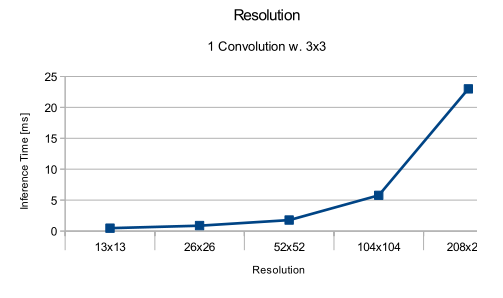
\includegraphics[width=\textwidth]{resolution_jevois.png}
	\end{minipage}
	\begin{minipage}{0.5\textwidth}
		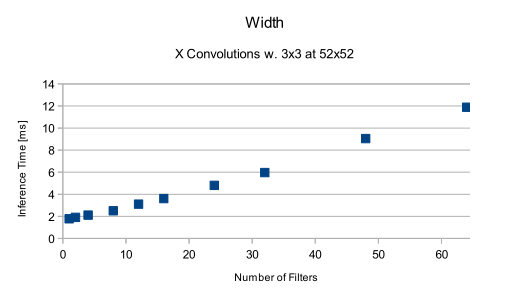
\includegraphics[width=\textwidth]{width_jevois.png}
\end{minipage}

	\begin{minipage}{0.5\textwidth}
		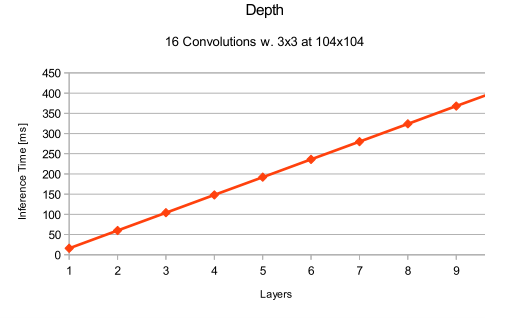
\includegraphics[width=\textwidth]{depth_jevois.png}
\end{minipage}
\label{fig:jevois}

\caption{Performance Measurements Darknet Jevois}
\end{figure}

In the graph for resolution and width we can see how the inference time increases with the number of computations. While slowly at first, at some point the increase is 1:1. Assumably this happens when the computations don't fit into one GPU cycle anymore. Unfortunately, this happens already at a resolution of 52x52. As we can see the computation time doubles when increasing to 104x104.
\newpage
\section{Crop and Refine approach}

In literature we find R-CNN, Fast-RCNN and Faster-RCNN as the second class of state-of-the art object detectors. Usually a classification network is modified such that the final layer proposes bounding boxes. This pretty similar to Yolo and SSD. A binary classification "object" or "no object" is done for a predefined and pre-parameterized set of so called anchor boxes.

The generated boxes are then fed to the second stage which classifies the object and refines the bounding box.
Initially an SVM or a second CNN was used for classification. Fast-RCNN introduced "ROI-Pooling" a layer which enables to pool from proposed bounding boxes to a predefined size. This enabled to pool from the last layer of the region proposal network and thus to reuse the filter outputs and use a very simple classifier. 

Generally, two stage detectors are more accurate but slower than single stage detectors like Yolo and SSD. Assumably because of the two stage character and because overlapping regions are processed multiple times in the classification stage. However, in our case we could merge overlapping regions and predict multiple boxes in the second stage. Also, we can run the proposal network less frequent than the refine network.

\subsection{ First stage}


In the first approach the region proposal stage is framed as classification task. A CNN applies convolutional- and pooling-layers until a certain grid size is reached e.g. 13x13, 6x6, 3x3. The filter maps are fed into a fully connected layer with sigmoid activation. Each grid cell is classified to "object" or "background". Unfortunately, this did not work at all. Even with 5 or 6 layers the accuracy did not exceed 50\%.

In the second approach anchor boxes are used for region proposal. Instead of predicting height and width, just a scale factor for each box is predicted. The target is defined as predicting a box 1.25 larger than the original label. Results of a 5-layer network can be seen in \autoref{fig:firststage}

\begin{figure}[h]
	\begin{minipage}{0.5\textwidth}
		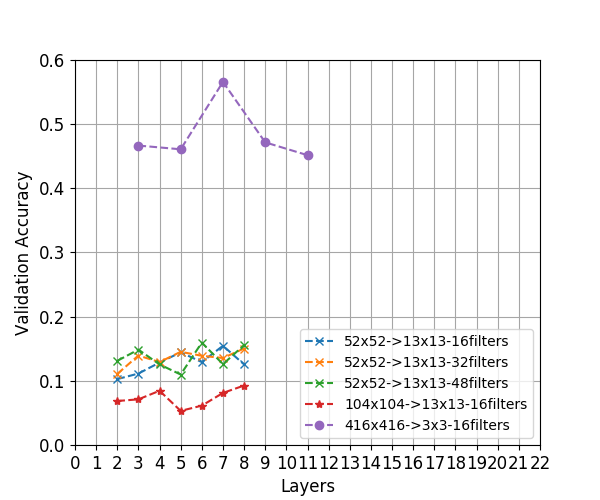
\includegraphics[width=\textwidth]{cropnet.png}
	\end{minipage}
	\begin{minipage}{0.5\textwidth}
		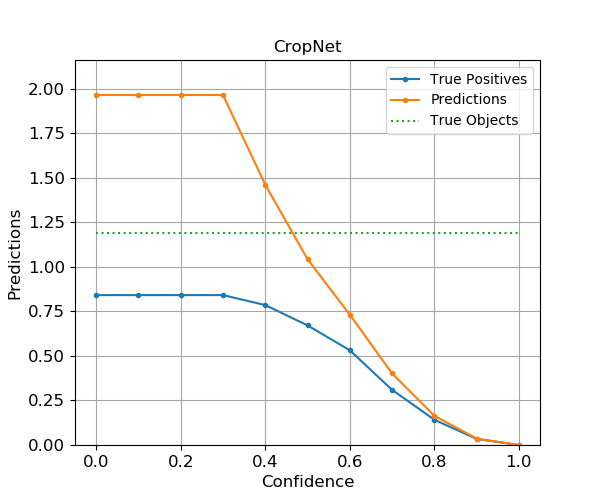
\includegraphics[width=\textwidth]{cropnet_predictions.png}
	\end{minipage}
	
	\label{fig:firststage}
	
	\caption{Results of the first stage. The testset consists of 1000 images. The results show the average per image.}
\end{figure}

For the first stage we want a high recall, so we can select all boxes with a confidence of more than 0.1 for the second stage. This will result in 2 regions per image on average. 

Based on the speed measurements taken out this network should require not more than 25ms. We could even run it only on every second or third frame as the gate position should not change too quickly.

In this configuration we should be able to run the second stage on all proposed regions. However, when there are more gates visible there might be too many proposed regions to examine all of them. In that case we would need to filter overlapping ones/ small boxes/boxes with low confidence.

\subsection{Second Stage}

In the second stage ROI-Pooling can be used to pool the input image from the proposed regions of the first stage to a fixed resolution. This has been implemented but is not really working yet. Currently the network is predicting nan after the first iteration.


\section{Quantization/Model Compression/Depthwise Separable Convolutions}

A lot of papers propose quantization to increase network speed for mobile devices. However, mostly they assume a CPU is used, which usually are not optimized for floating point operations. In our case we use a GPU which is optimized for floating point operations. So quantization would not necessarily increase speed.

Model compression mostly aims at reducing the width of large networks to smaller networks. However, our current best model is already only 64 filters wide at max. So its questionable whether we can make it much thinner.

Depthwise Separable Convolutions are often used to reduce the number of computations e.g. MobileNet/ShuffleNet. Apparently they don't seem to work that well on small networks and also when I ran one test with them performance really broke down. Still it might be worth a second look.

\section{Conclusion}
\begin{itemize}
	\item Darknet enables us to use the GPU and run networks faster. However, we still can't process the image at full resolution.
	\item The two-stage approaches deliver a framework for our course-to-fine approach.
	\item In the first stage a 5-layer network seems to be enough to propose regions.
\end{itemize}

\section{Next Steps}
\begin{itemize}
	\item Write it all down.
	\item Finish implementation with two stage approach.
	\item Implement it in darknet.
	\item Investigate effect of depthwise separable convolutions on performance and speed.
	
\end{itemize}


\end{document}\grid
